The first point on which we worked was to find a way of building a map of the environment of the robot using the lasers echoes.

To do so we created a class 'Map' that contains a grid of values between $0$ and $1$.
Those values represent probability that there is an obstacle on that cell.
All the values are initialized to $0.5$ which is the average value between $0$ and $1$ since we do not know if there is an obstacle or not at that place.

To update this grid we created a class 'Cartographer' that uses the echoes of the lasers.
For each laser echoe we compute the distance between the robot cell and the cell hit by the laser in the grid.
Then we use the 'Bresenham' algorithm\cite{bresenham} to update all the cells in between the two above.
For all those cells we compute an increment that is added or subtracted to them using the following procedure:

\begin{enumerate}
    \item First we compute an increment value in regard of the value of the cell, the values for max and min increments are respectfully 0.15 and 0.015:
        \begin{itemize}
            \item[$-$] If the cell is a hit cell, meaning that it is the cell where the laser echoed back:
            $$
                inc\_iro\_certainty = min\_increment\texttt{ if }is\_empty(cell)\texttt{ else }max\_increment
            $$
            \item[$-$] If the cell is not a hit cell:
            $$
                inc\_iro\_certainty = min\_increment\texttt{ if }is\_obstacle(cell)\texttt{ else }max\_increment
            $$
        \end{itemize}
    \item Then we compute an increment factor in regard of the distance between the robot and the cell to update:
        $$
        inc\_factor\_iro\_dist = 1 - abs(\dfrac{distance}{max\_lasers\_distance})
        $$
    \item The final increment is computed by multiplying the factor with the defined increment:
        $$
        final\_increment = inc\_iro\_certainty \cdot inc\_factor\_iro\_dist
        $$
    \item The final increment is added to the cell if the cell corresponds to the cell hit by the laser and that the distance of the echoe is below the maximum laser distance.
        Otherwise it is subtracted.
\end{enumerate}

With this method when a cell is qualified as obstacle it will be 10 times harder to decrement its value than to increment it and reversely.
That makes the map more consistent because even when the robot hits something which make it shake or turns very fast we will not have false values in our grid.
The distance factor is useful because it will make the cells near the robot update more easily than the cells far away, since the further away the cell is from the robot the less precise the laser information is.

This is the factory map built moving the robot by hand using the cartographer described above.

\FloatBarrier
\begin{figure}
    \centering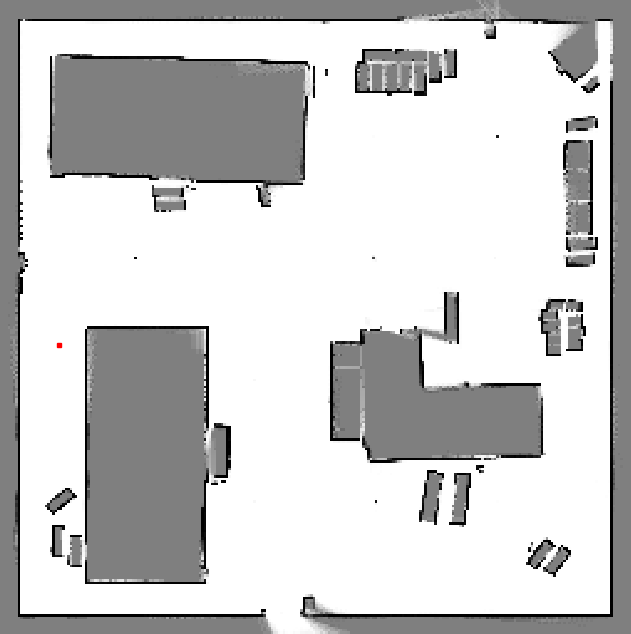
\includegraphics[width=\textwidth]{explored_map_by_hand.png}
    \label{fig:explored_map_by_hand}
    \caption{Explored map by hand}
\end{figure}
\FloatBarrier

The mapping module also contains the 'ShowMap' class which is used to display the built map.
